\section{Principal Component Analysis (PCA)}

\begin{frame}{Learning Goals}
\begin{itemize}
  \pause
  \item Start from a centered data matrix and a projection direction.
  \pause
  \item Derive PCA as variance maximization under a unit-norm constraint.
  \pause
  \item Connect the optimization problem to eigenvectors, eigenvalues, and orthogonality.
  \pause
  \item Understand practical computation with covariance, power iteration, deflation, and SVD.
  \pause
  \item Use PCA for compression, visualization, and anomaly detection.
\end{itemize}
\end{frame}

\begin{frame}{Data Matrix and Projection}
\begin{columns}[T]
\column{0.55\textwidth}
\begin{itemize}
  \item Assume centered data stacked in $X_c \in \mathbb{R}^{n\times d}$.
  \pause
  \item Choose a direction $w \in \mathbb{R}^d$.
  \pause
  \item Each sample projects to one scalar $z_i = w^\top x_i$.
  \pause
  \item For the whole data set, $z = X_c w \in \mathbb{R}^n$ collects all projected coordinates.
  \pause
  \item PCA asks which direction keeps the largest spread after this projection.
\end{itemize}

\pause
\column{0.45\textwidth}
\centering
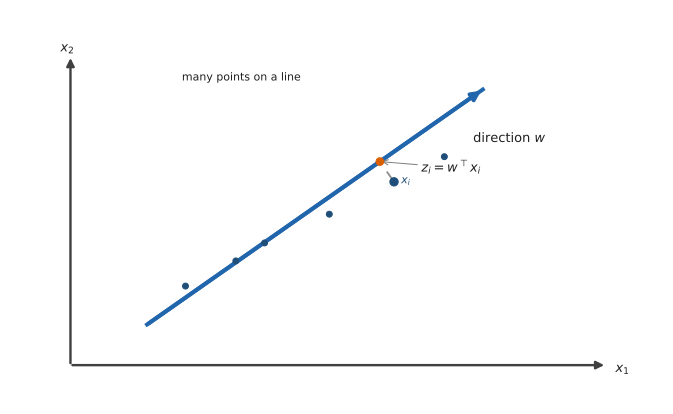
\includegraphics[width=\textwidth]{figures/pca/pca_projection.pdf}
\end{columns}
\end{frame}

\begin{frame}{Projected Variance}
\begin{itemize}
  \item The projected scalars are $z_i = w^\top x_i$.
  \pause
  \item Because the data are centered, the projected mean is also zero.
  \pause
  \item So the variance of the projection is
  \begin{equation}
    \mathrm{Var}(w^\top x)
    = \frac{1}{n-1}\sum_{i=1}^{n}(w^\top x_i)^2
    = \frac{1}{n-1}\sum_{i=1}^{n} w^\top x_i x_i^\top w
    = w^\top \Sigma w,
    \label{eq:proj-var-pca}
  \end{equation}
  where
  \[
    \Sigma = \frac{1}{n-1}X_c^\top X_c.
  \]
  \pause
  \item PCA now chooses the direction that maximizes $w^\top \Sigma w$.
\end{itemize}
\end{frame}

\begin{frame}{PCA as a Constrained Problem}
\begin{itemize}
  \item The first principal direction solves
  \begin{equation}
    \max_{w} \; w^\top \Sigma w
    \quad \text{subject to} \quad
    w^\top w = 1.
    \label{eq:pca-constrained}
  \end{equation}
  \pause
  \item The unit-norm constraint fixes scale.
  \pause
  \item Without it, multiplying $w$ by a constant would change the objective artificially.
\end{itemize}
\end{frame}

\begin{frame}{From Optimization to Eigenvectors}
\begin{itemize}
  \item Introduce a Lagrange multiplier $\lambda$:
  \begin{equation}
    \mathcal{L}(w,\lambda)=w^\top \Sigma w-\lambda (w^\top w-1).
    \label{eq:lagrangian}
  \end{equation}
  \pause
  \item Differentiate with respect to $w$:
  \begin{equation}
    \nabla_w \mathcal{L}(w,\lambda)=2\Sigma w-2\lambda w = 0.
    \label{eq:lagrange-grad}
  \end{equation}
  \pause
  \item Rearranging gives the eigenvalue equation:
  \begin{equation}
    \Sigma w = \lambda w.
    \label{eq:eigenproblem-pca}
  \end{equation}
  \item So PCA directions are eigenvectors of the covariance matrix.
\end{itemize}
\end{frame}

\begin{frame}{A Better Basis for the Argument}
\begin{itemize}
  \item The covariance matrix $\Sigma$ is symmetric.
  \pause
  \item Therefore its eigenvectors can be chosen orthonormal:
  \[
    v_i^\top v_j =
    \begin{cases}
      1, & i=j,\\
      0, & i\neq j.
    \end{cases}
  \]
  \pause
  \item That means any unit vector $w$ can be written in this basis:
  \begin{equation}
    w = \sum_{j=1}^d \alpha_j v_j,
    \qquad \sum_{j=1}^d \alpha_j^2 = 1.
    \label{eq:eigenbasis-expansion}
  \end{equation}
  \pause
  \item Now we can study the PCA objective by looking at the coefficients $\alpha_j$.
\end{itemize}
\end{frame}

\begin{frame}{Why the Largest Eigenvalue Wins}
\small
\begin{itemize}
  \item Let $v_1,\dots,v_d$ be eigenvectors of $\Sigma$ with
  $\lambda_1\ge \lambda_2 \ge \cdots \ge \lambda_d$.
  \pause
  \item Start from the PCA objective:
  \begin{equation}
    w^\top \Sigma w.
    \label{eq:pca-objective-short}
  \end{equation}
  \pause
  \item Substitute $w=\sum_j \alpha_j v_j$ and use $\Sigma v_j=\lambda_j v_j$:
  \begin{equation}
    w^\top \Sigma w = \sum_{j=1}^d \lambda_j \alpha_j^2.
    \label{eq:weighted-eigenvalues}
  \end{equation}
  \pause
  \item Cross-terms vanish because the eigenvectors are orthonormal.
  \pause
  \item So the variance is a weighted average of the eigenvalues, with weights $\alpha_j^2$.
  \pause
  \item In 2D, if $w=\cos\theta\, v_1+\sin\theta\, v_2$, then
  \[
    w^\top \Sigma w = \lambda_1\cos^2\theta + \lambda_2\sin^2\theta.
  \]
  The closer $w$ is to $v_1$, the more weight goes to $\lambda_1$.
\end{itemize}
\end{frame}

\begin{frame}{Why the Maximum Is $\lambda_1$}
\small
\begin{itemize}
  \item Since the weights are nonnegative and sum to $1$,
  \begin{equation}
    w^\top \Sigma w = \sum_{j=1}^d \lambda_j \alpha_j^2 \le \lambda_1.
    \label{eq:max-eigenvalue}
  \end{equation}
  \pause
  \item A weighted average cannot be larger than its largest entry.
  \pause
  \item Equality holds only when $\alpha_1=1$ and all other $\alpha_j=0$.
  \pause
  \item So the maximizing direction is $w=v_1$.
\end{itemize}
\end{frame}

\begin{frame}{Why There Are Several Principal Components}
\begin{columns}[T]
\column{0.56\textwidth}
\begin{itemize}
  \item The first component maximizes variance with no other constraint.
  \pause
  \item The second component maximizes variance subject to orthogonality to the first.
  \pause
  \item In general,
  \begin{equation}
    w_k = \arg\max_{\|w\|_2=1,\; w^\top w_j=0\ \forall j<k} w^\top \Sigma w.
    \label{eq:pk}
  \end{equation}
  \pause
  \item This gives orthogonal directions of decreasing variance.
\end{itemize}

\pause
\column{0.44\textwidth}
\centering
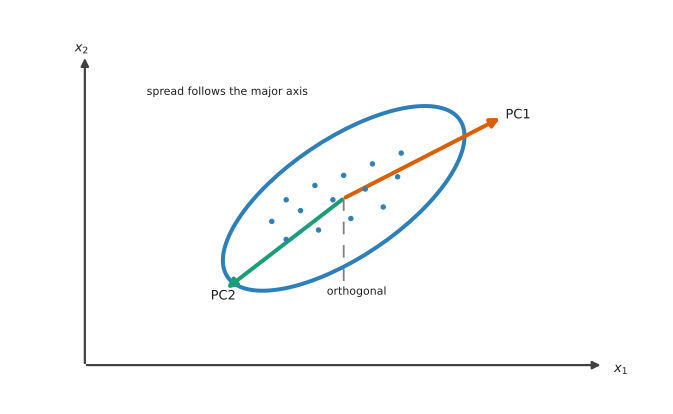
\includegraphics[width=\textwidth]{figures/pca/pca_axes.pdf}
\end{columns}
\end{frame}

\begin{frame}{Power Iteration}
\begin{itemize}
  \item One practical way to find the top eigenvector is power iteration:
  \begin{equation}
    v^{(t+1)} = \frac{\Sigma v^{(t)}}{\|\Sigma v^{(t)}\|_2}.
    \label{eq:power-iteration}
  \end{equation}
  \pause
  \item Repeated multiplication amplifies the dominant eigen-direction.
  \pause
  \item The vector is renormalized after every step.
  \pause
  \item This is useful for intuition and for the top component.
\end{itemize}
\end{frame}

\begin{frame}{Deflation for Later Components}
\begin{itemize}
  \item After finding $w_1$ and $\lambda_1$, remove its contribution:
  \begin{equation}
    \Sigma_2 = \Sigma - \lambda_1 w_1 w_1^\top.
    \label{eq:deflation}
  \end{equation}
  \pause
  \item Then apply the same procedure to $\Sigma_2$ to get the next direction.
  \pause
  \item This enforces orthogonality and prevents rediscovering the first component.
\end{itemize}
\end{frame}

\begin{frame}{Why Libraries Use SVD}
\begin{itemize}
  \item The covariance route first builds
  \[
    \Sigma = \frac{1}{n-1}X_c^\top X_c.
  \]
  \pause
  \item In practice, libraries often avoid forming $\Sigma$ explicitly.
  \pause
  \item Forming $X_c^\top X_c$ adds an extra matrix multiplication and can amplify numerical error.
  \pause
  \item So many libraries work directly with the centered data matrix $X_c$.
\end{itemize}
\end{frame}

\begin{frame}{SVD Gives the Same PCA Directions}
\begin{itemize}
  \item Factor the centered data matrix directly:
  \begin{equation}
    X_c = U S V^\top.
    \label{eq:svd-pca}
  \end{equation}
  \pause
  \item Then
  \begin{equation}
    X_c^\top X_c = V S^\top S V^\top = V S^2 V^\top.
    \label{eq:xtx}
  \end{equation}
  \pause
  \item So the columns of $V$ are the same principal directions we obtained from the covariance eigenproblem.
  \pause
  \item The squared singular values $s_j^2$ are proportional to explained variances.
\end{itemize}
\end{frame}

\begin{frame}{What the SVD Factors Mean for PCA}
\begin{itemize}
  \item $V$ contains the principal directions in feature space.
  \pause
  \item $X_cV$ gives the data expressed in principal-component coordinates.
  \pause
  \item Since $X_c = U S V^\top$, multiplying by $V$ gives
  \[
    X_cV = US.
  \]
  \pause
  \item So SVD gives both the PCA directions ($V$) and the sample coordinates along them ($US$).
\end{itemize}
\end{frame}

\begin{frame}{SVD Geometry}
\begin{columns}[T]
\column{0.58\textwidth}
\begin{itemize}
  \item SVD decomposes the data into rotation, stretching, and rotation:
  \[
    X_c = U S V^\top.
  \]
  \pause
  \item $V^\top$ rotates feature axes into principal directions.
  \pause
  \item $S$ stretches or shrinks along those directions.
  \pause
  \item $U$ organizes the sample coordinates after that transformation.
  \pause
  \item This is why SVD is numerically stable and widely used.
\end{itemize}
\pause
\column{0.42\textwidth}
\centering
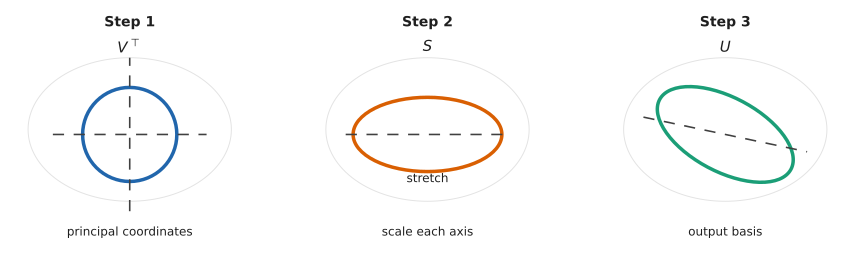
\includegraphics[width=\textwidth]{figures/pca/pca_svd_geometry.pdf}
\end{columns}
\end{frame}

\begin{frame}{Geometric Intuition}
\begin{columns}[T]
\column{0.56\textwidth}
\begin{itemize}
  \item PCA finds the axes of maximal stretching in the data cloud.
  \pause
  \item The first axis is the direction of largest variance.
  \pause
  \item The second axis is orthogonal and captures the next largest remaining variance.
  \pause
  \item SVD gives the same axes through a stable matrix factorization.
\end{itemize}
\pause
\column{0.44\textwidth}
\centering
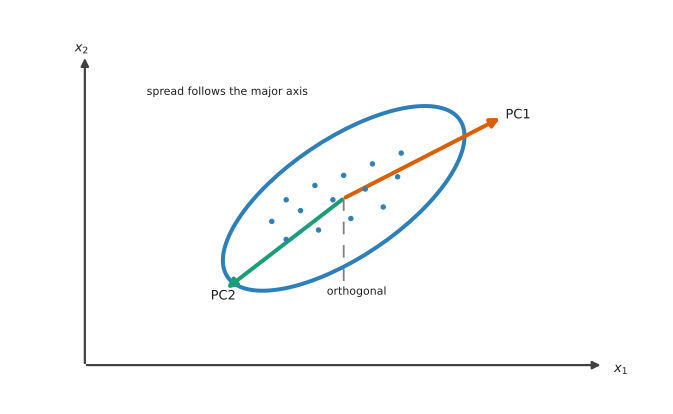
\includegraphics[width=\textwidth]{figures/pca/pca_axes.pdf}
\end{columns}
\end{frame}

\begin{frame}{Summary}
\begin{itemize}
  \item PCA starts with projection and asks for the direction with maximum projected variance.
  \item The optimization becomes an eigenvalue problem through a constrained quadratic form.
  \item The largest eigenvector gives the first principal component; the rest follow by orthogonality.
  \item In practice, PCA is computed either from the covariance matrix or from SVD.
  \item The geometry is simple: rotate, stretch, keep the important axes.
\end{itemize}
\end{frame}

\begin{frame}{Next Lab}
\begin{itemize}
  \item Implement PCA from scratch with NumPy using both covariance eigendecomposition and SVD.
  \item Reuse the text-embedding setting from Lab 1 and visualize the embeddings in 2D with PCA.
  \item Compare k-NN on raw features versus PCA-reduced features on one earlier classification or regression task.
  \item Use PCA reconstruction error for anomaly detection and compare it with the k-NN anomaly score from Lab 1.
  \item Report what is gained and what is lost after dimensionality reduction: runtime, visualization, denoising, and predictive accuracy.
\end{itemize}
\end{frame}
